% !TEX TS-program = xelatex
% !TEX encoding = UTF-8
% !Mode:: "TeX:UTF-8"

\documentclass[onecolumn,oneside]{BUPTHomework}

\author{胡玉斌}
\sid{2021111054}
\title{cs155-proj3}
\coursecode{}
\coursename{网络安全}

\begin{document}
  \maketitle

  \section*{Part 0: Go Tutorial}

  
  \begin{lstlisting}
package main

import "fmt"

func main() {
    fmt.Println("Hello World")
}
  \end{lstlisting}

  \begin{figure}[h]
    \centering
    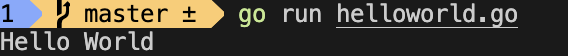
\includegraphics[width=0.70\textwidth]{img/fig1.png}
    \caption{helloworld}
    \label{fig1}
  \end{figure}
  
  \section*{Part 1: Nmap Port Scanning}

  \begin{figure}[h]
    \centering
    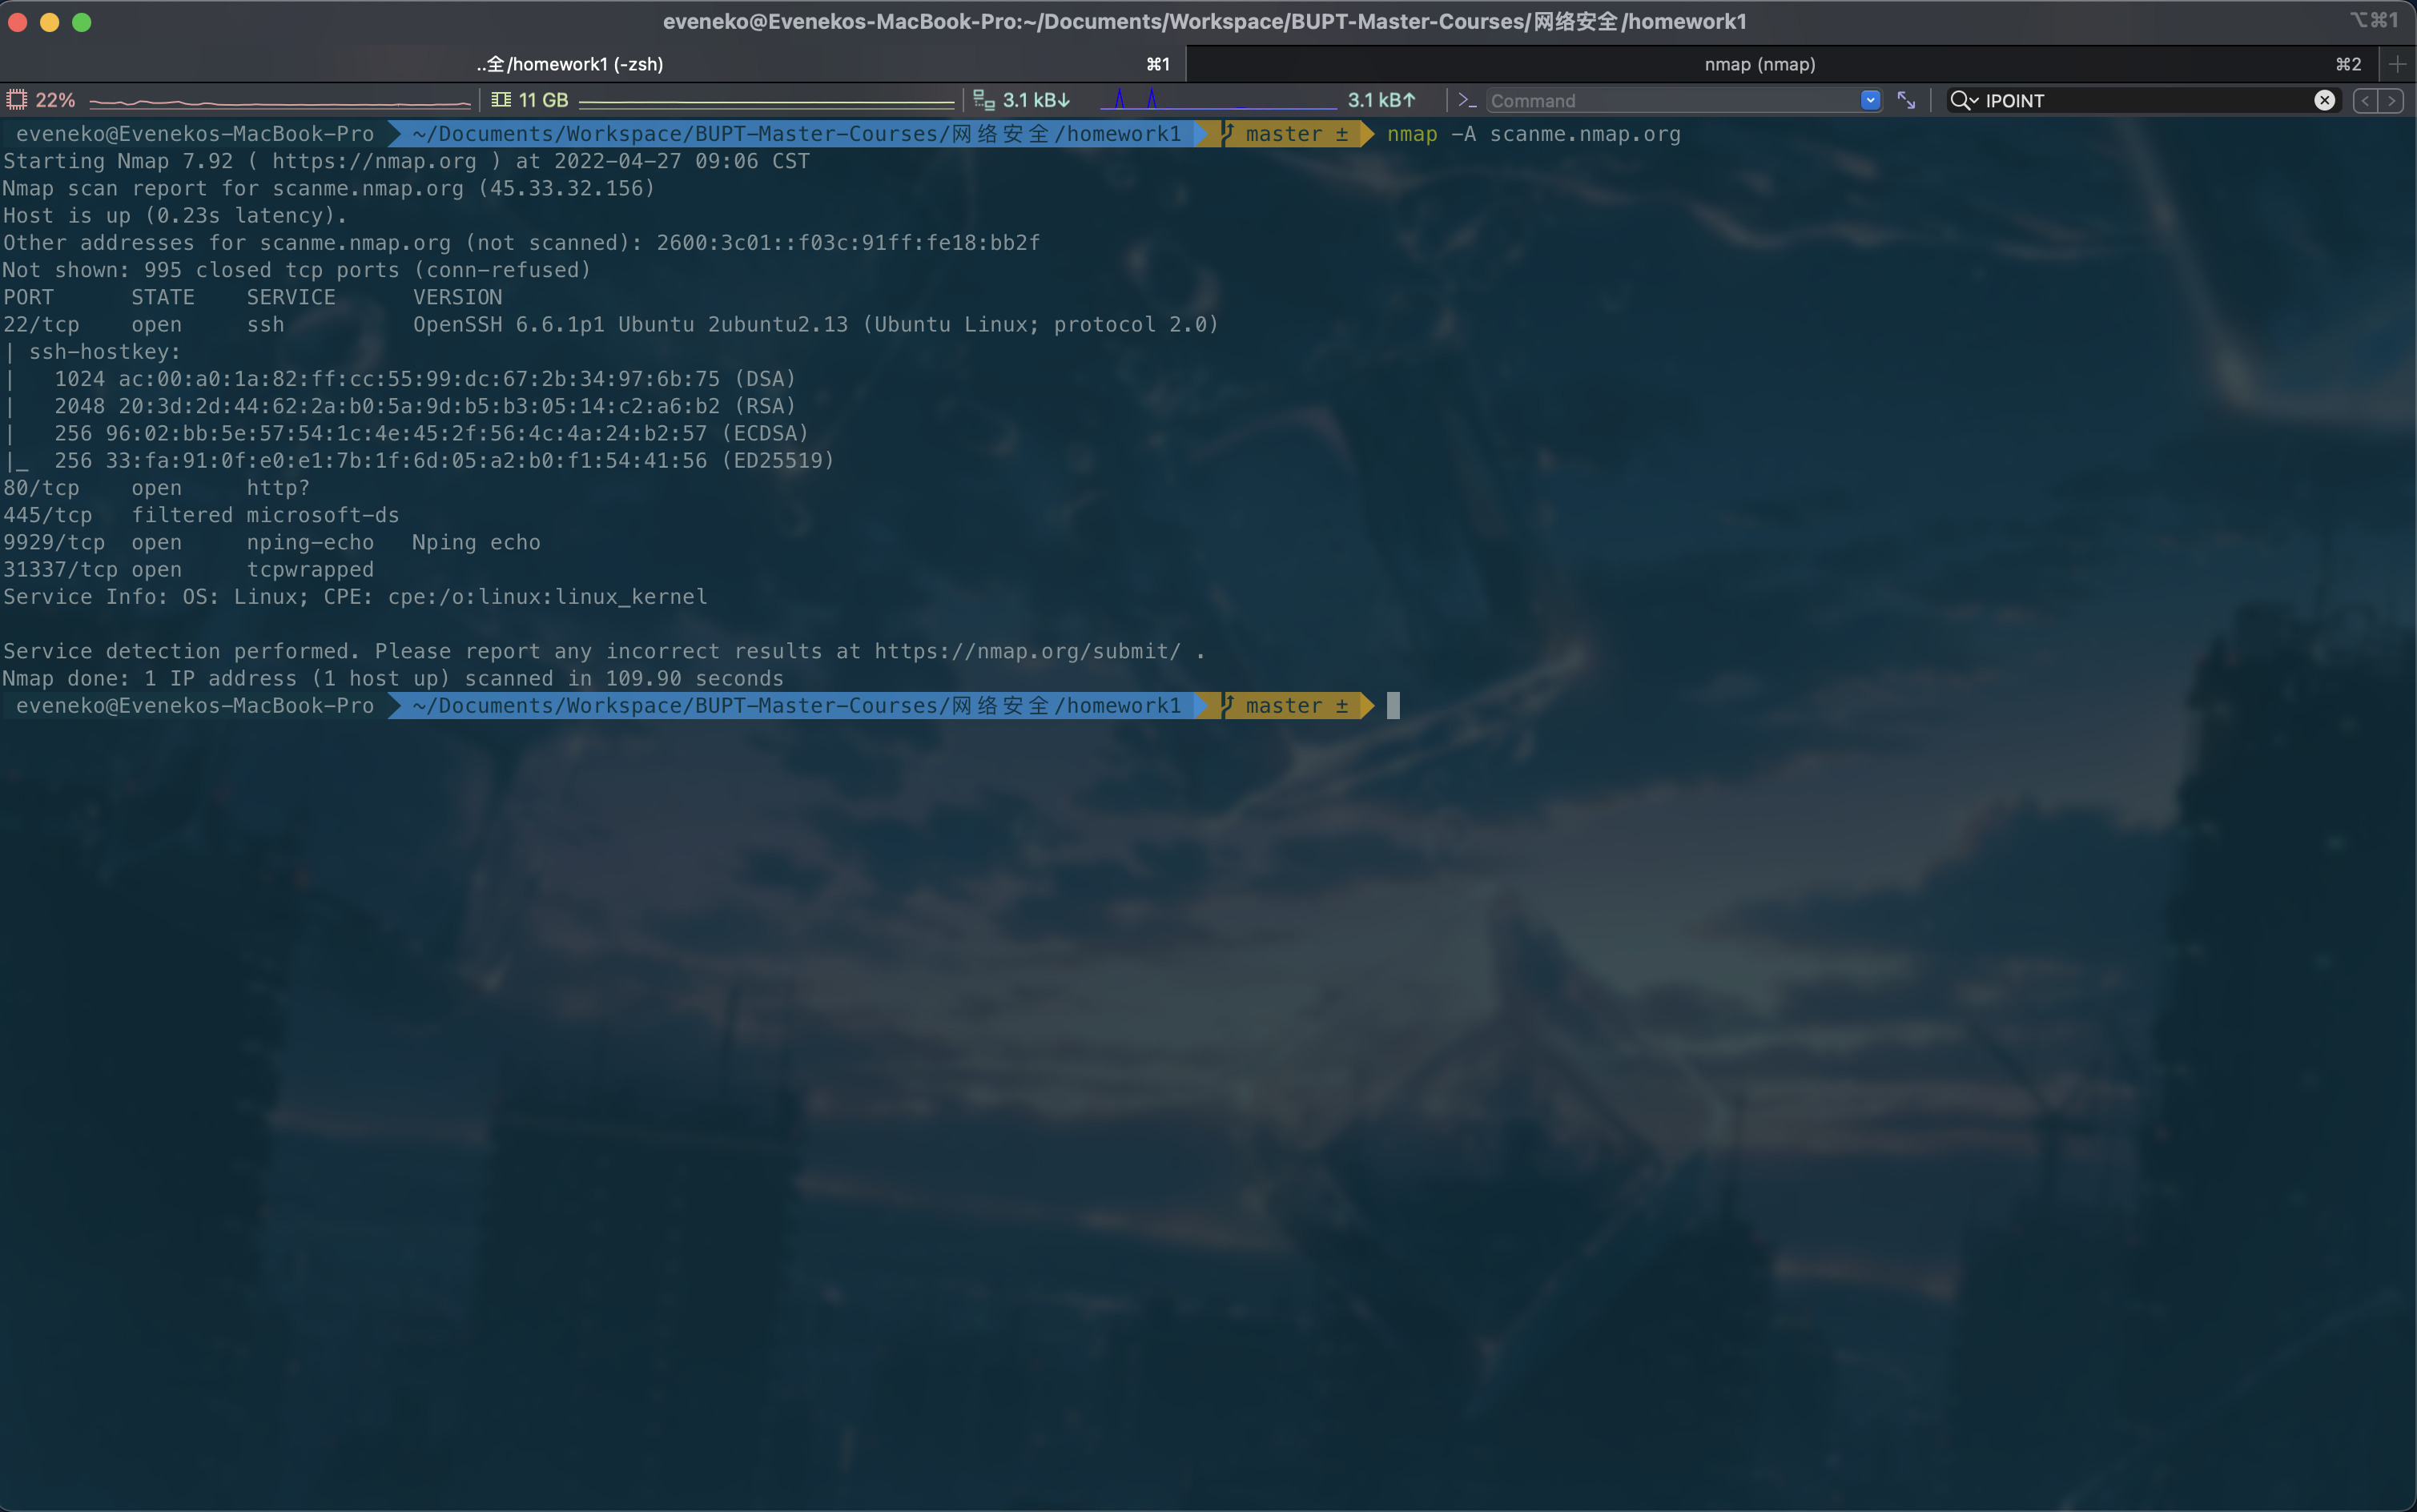
\includegraphics[width=1.00\textwidth]{img/fig2.png}
    \caption{OS detection: nmap -A scanme.nmap.org}
    \label{fig2}
  \end{figure}

  \begin{figure}[h]
    \centering
    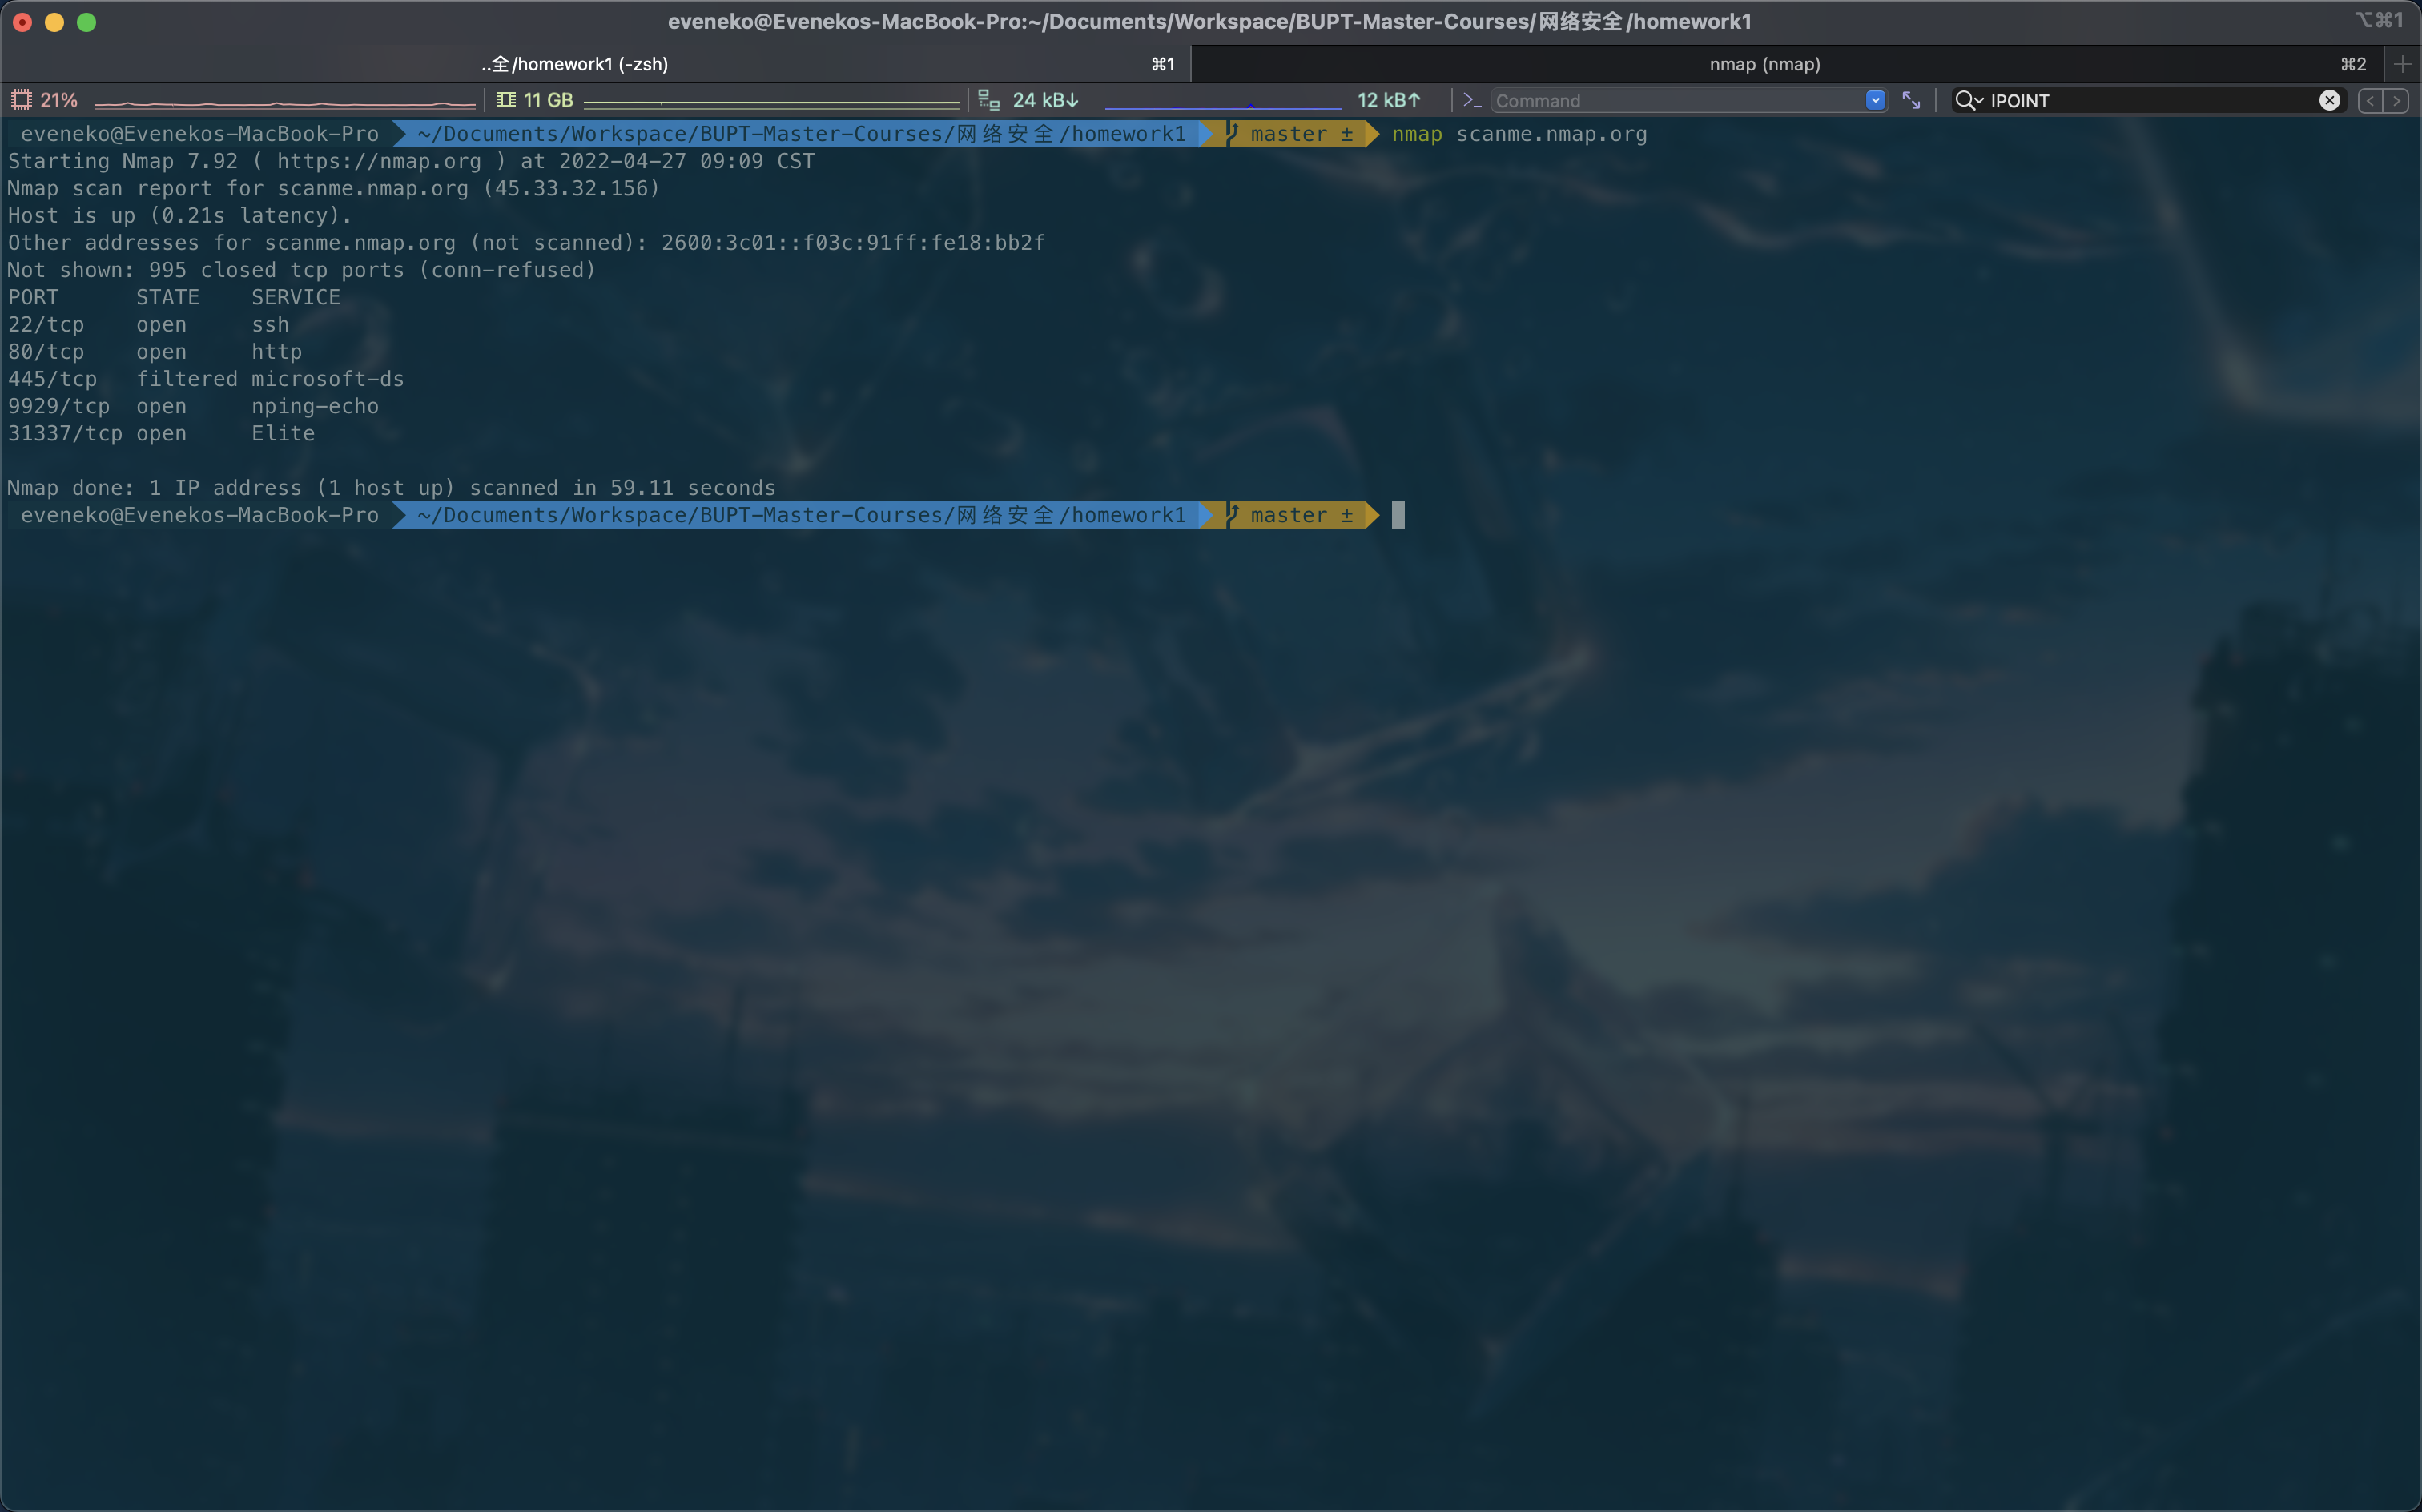
\includegraphics[width=1.00\textwidth]{img/fig3.png}
    \caption{nmap scanme.nmap.org}
    \label{fig3}
  \end{figure}

  \begin{figure}[h]
    \centering
    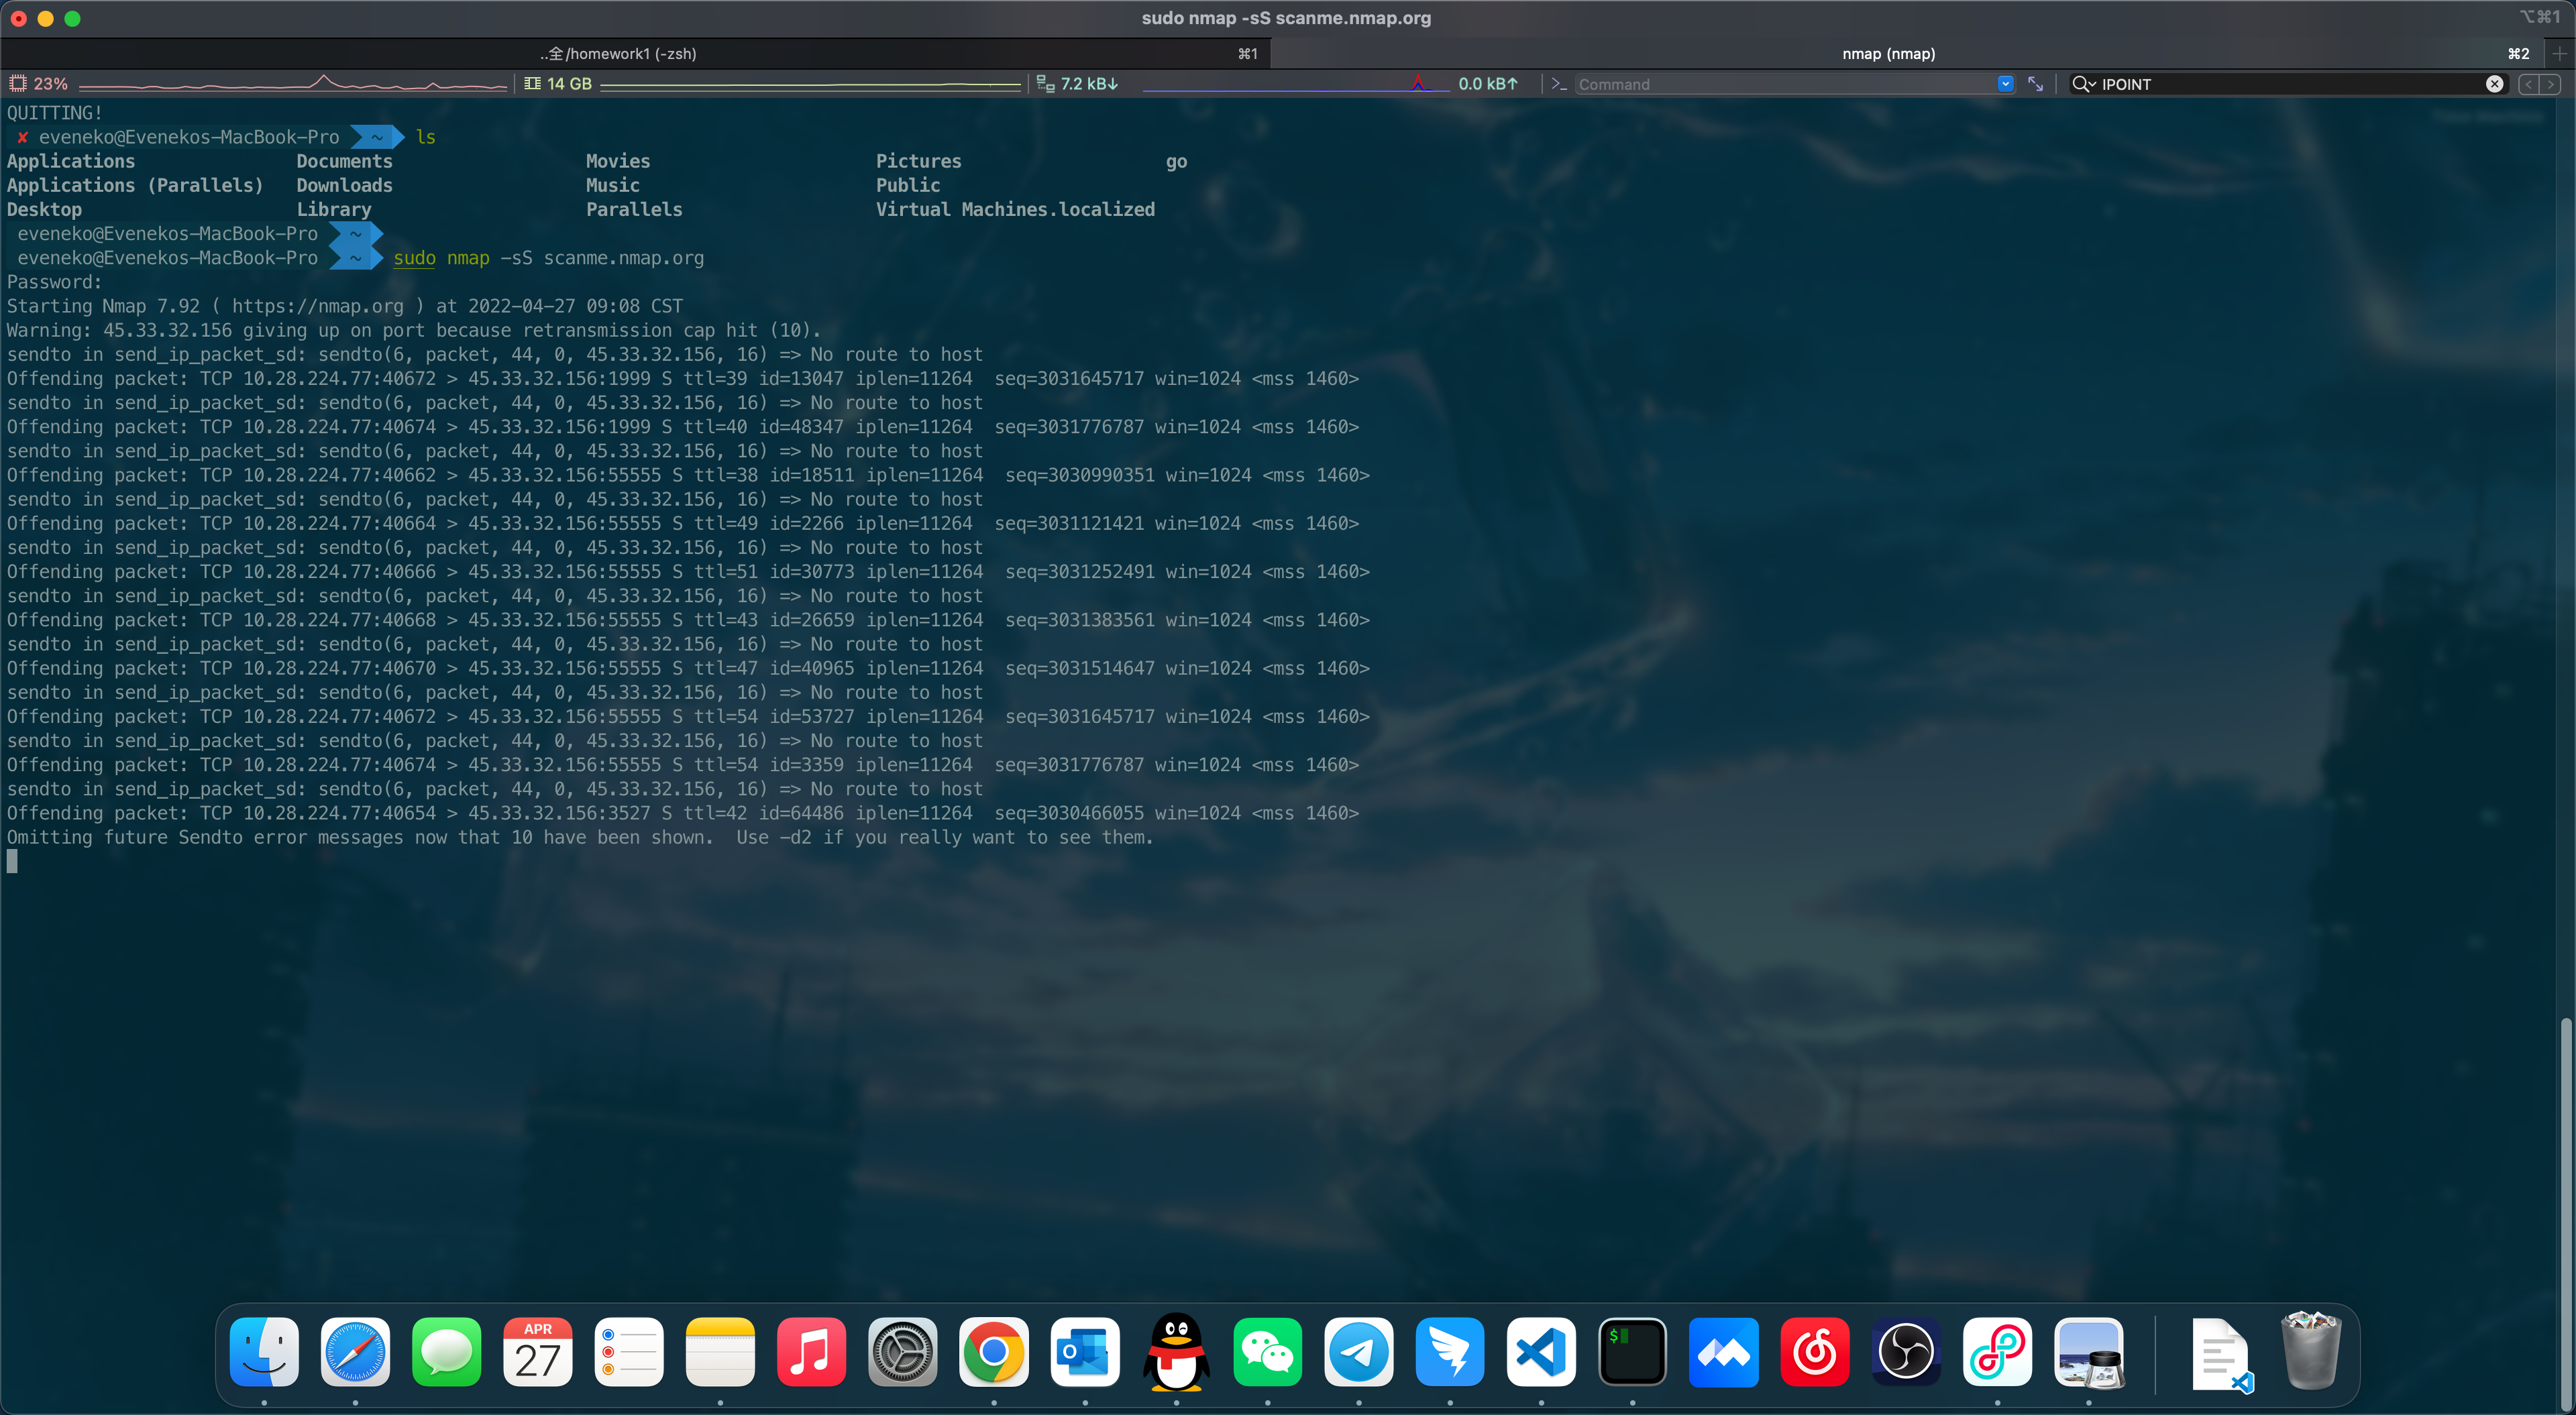
\includegraphics[width=1.00\textwidth]{img/fig4.png}
    \caption{TCP SYN scan: nmap -sS scanme.nmap.org}
    \label{fig4}
  \end{figure}

  \begin{figure}[h]
    \centering
    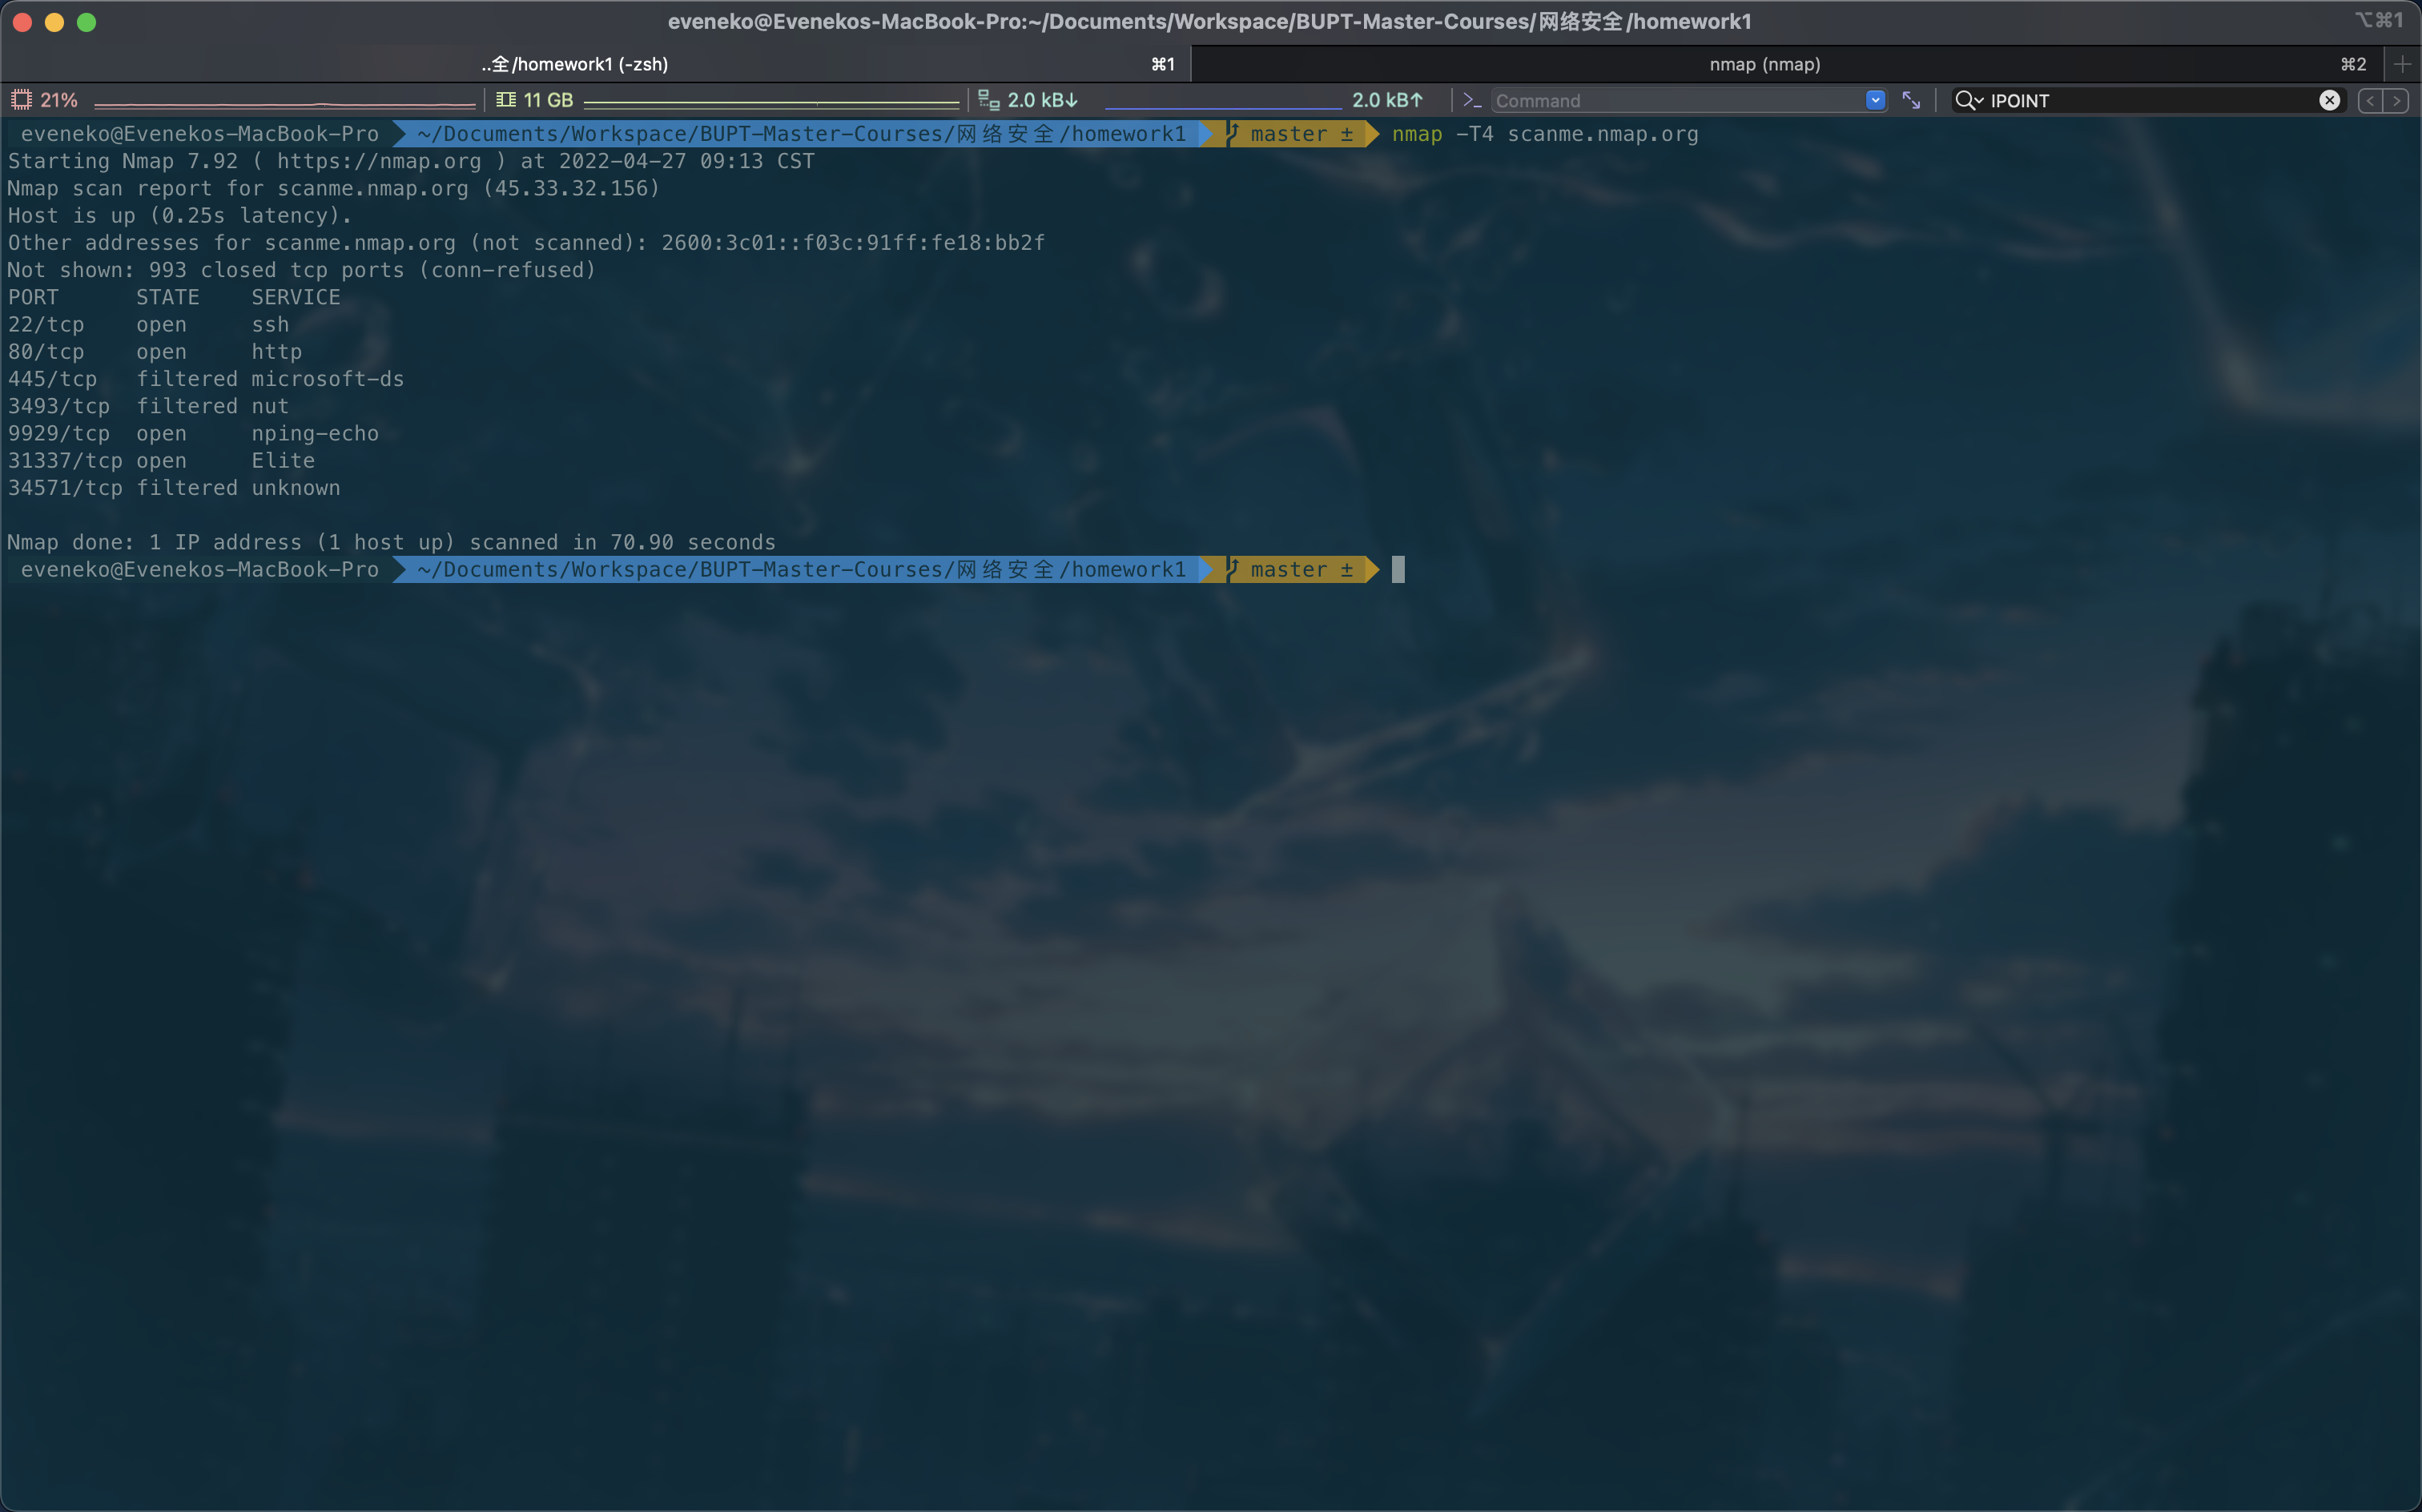
\includegraphics[width=1.00\textwidth]{img/fig5.png}
    \caption{nmap -T4 scanme.nmap.org}
    \label{fig5}
  \end{figure}

  \section*{Part 2: Wireshark Packet Sniffing}

  \begin{figure}[h]
    \centering
    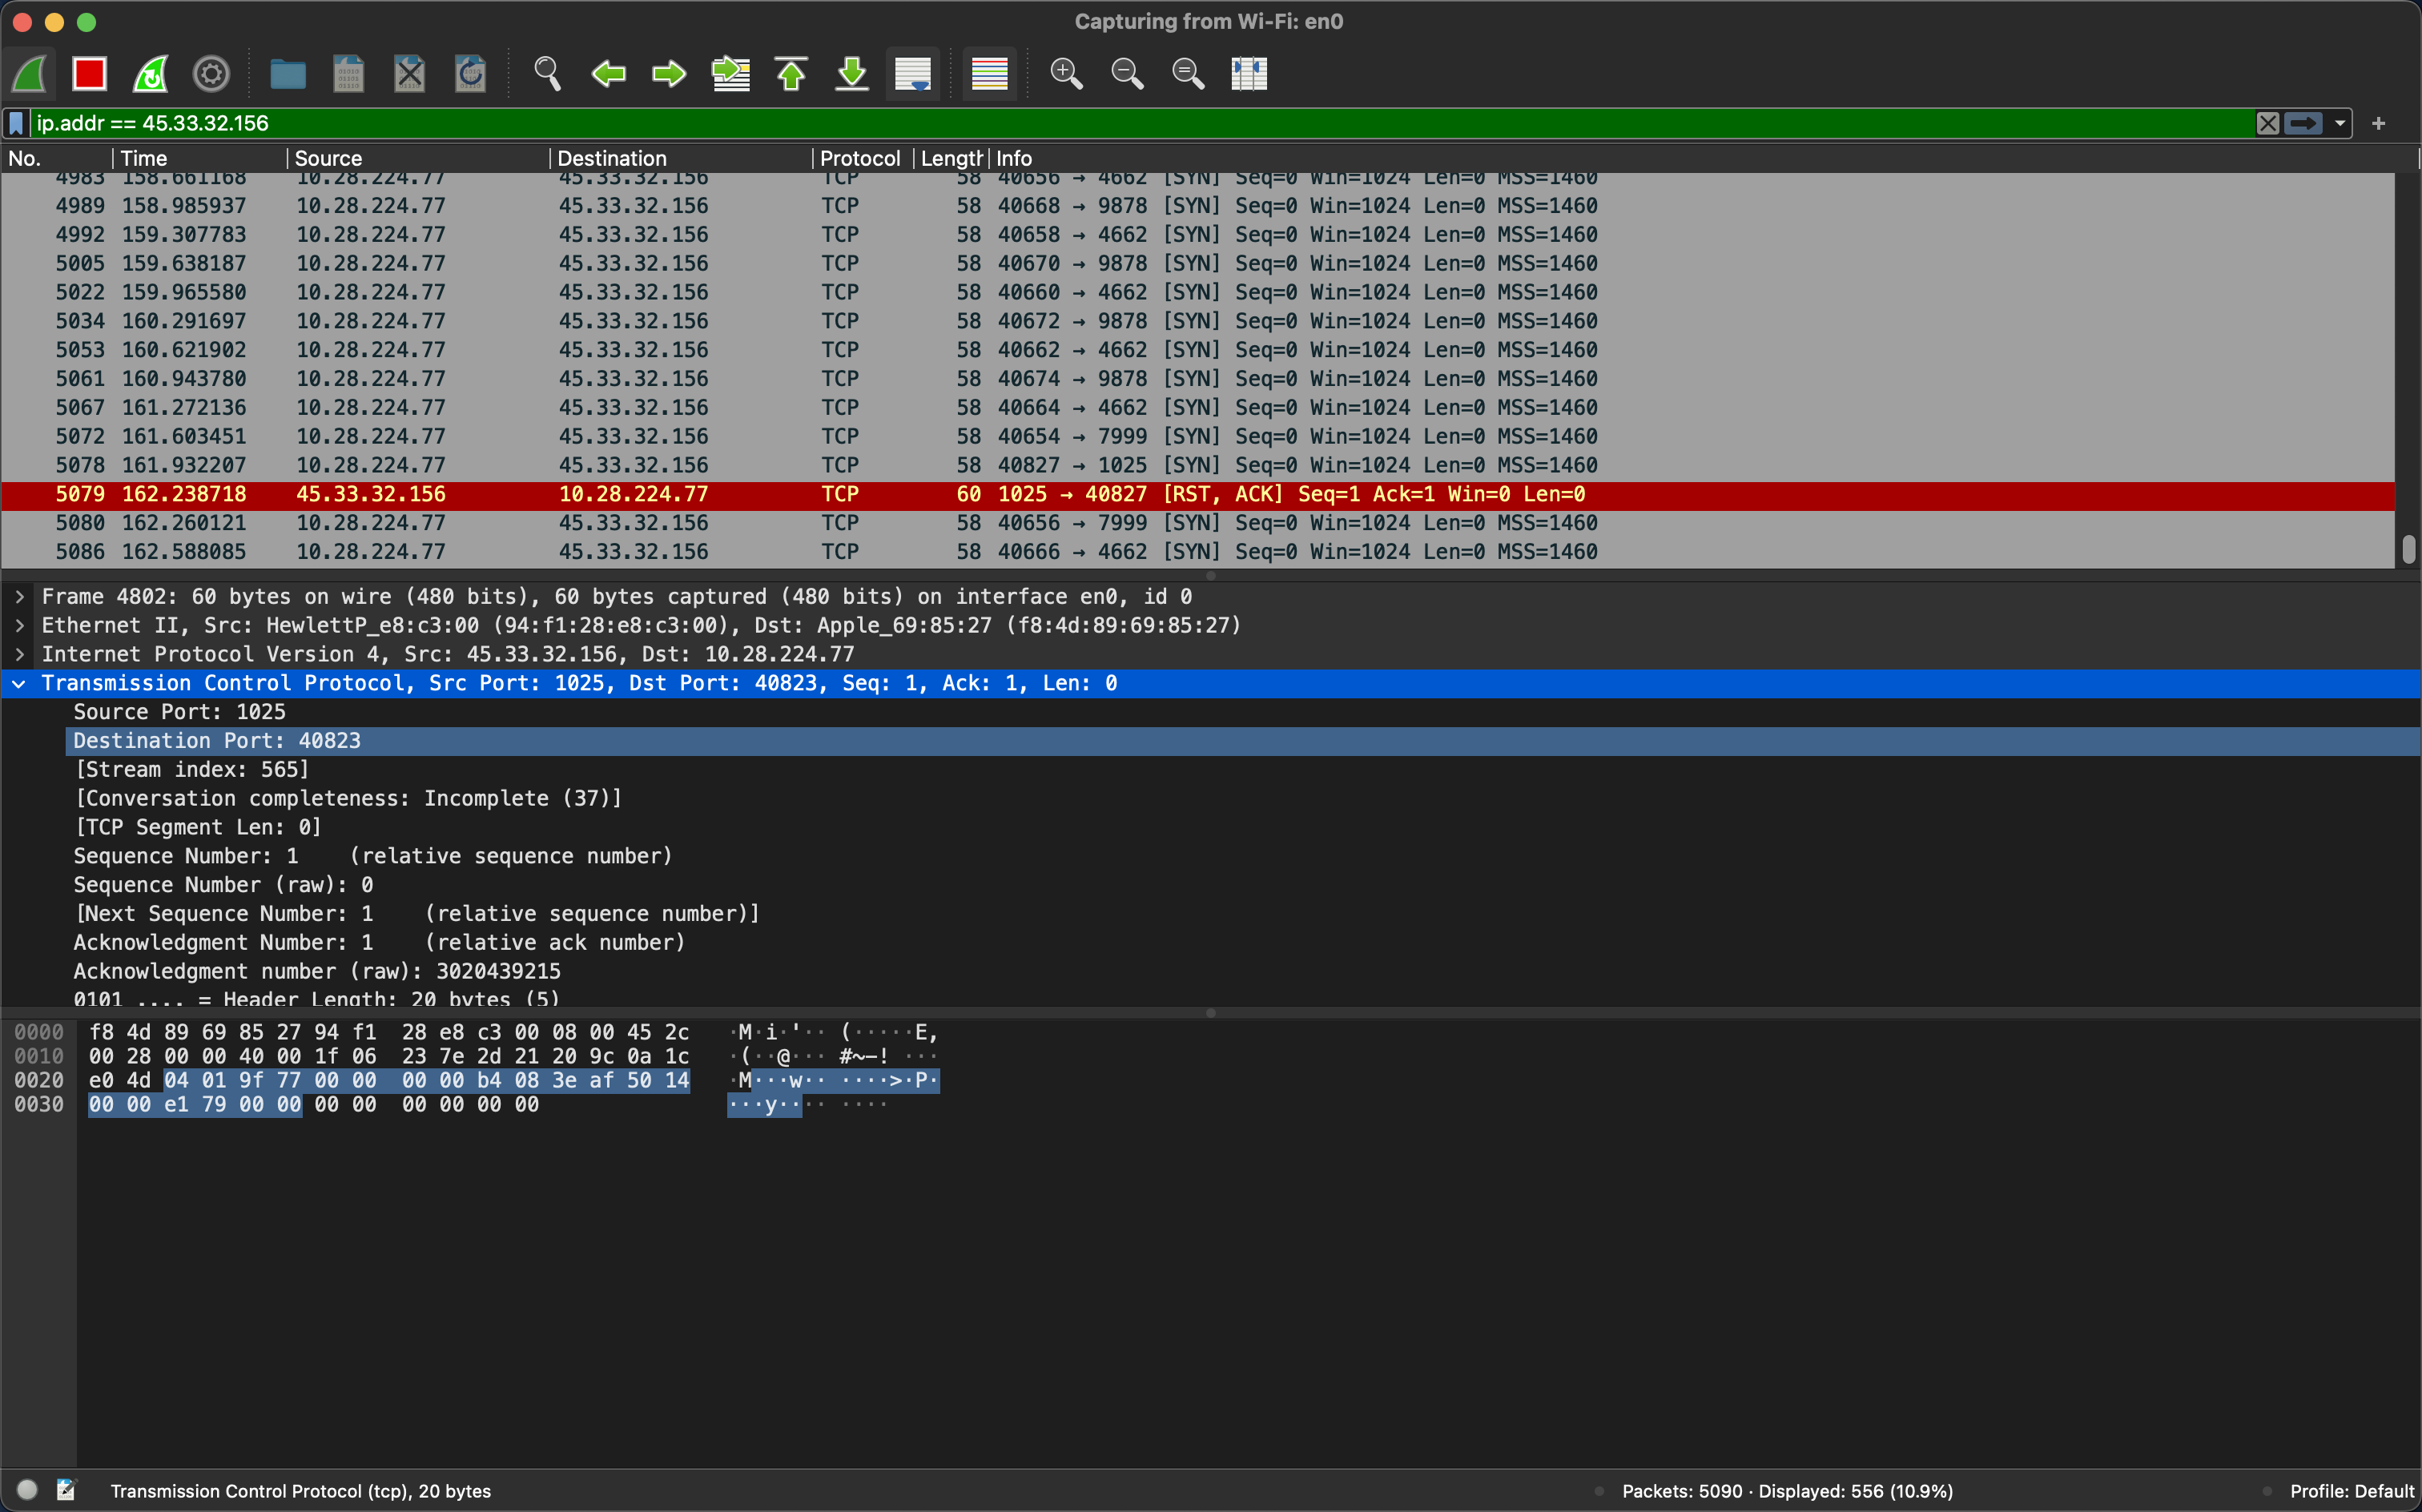
\includegraphics[width=1.00\textwidth]{img/fig6.png}
    \caption{Wireshark}
    \label{fig6}
  \end{figure}

  \section*{Part 3: Programmatic Packet Processing}

  \section*{Part 4: Monster-in-the-Middle Attack}

\end{document}
